
\documentclass[a4paper,11pt]{article}
\usepackage[a4paper, margin=8em]{geometry}

% usa i pacchetti per la scrittura in italiano
\usepackage[french,italian]{babel}
\usepackage[T1]{fontenc}
\usepackage[utf8]{inputenc}
\frenchspacing 

% usa i pacchetti per la formattazione matematica
\usepackage{amsmath, amssymb, amsthm, amsfonts}

% usa altri pacchetti
\usepackage{gensymb}
\usepackage{hyperref}
\usepackage{standalone}

\usepackage{colortbl}

\usepackage{xstring}
\usepackage{karnaugh-map}

% imposta il titolo
\title{Embedded Operating Systems and Architectures notes}
\author{Luca Seggiani}
\date{2026}

% imposta lo stile
% usa helvetica
\usepackage[scaled]{helvet}
% usa palatino
\usepackage{palatino}
% usa un font monospazio guardabile
\usepackage{lmodern}

\renewcommand{\rmdefault}{ppl}
\renewcommand{\sfdefault}{phv}
\renewcommand{\ttdefault}{lmtt}

% circuiti
\usepackage{circuitikz}
\usetikzlibrary{babel}

% testo cerchiato
\newcommand*\circled[1]{\tikz[baseline=(char.base)]{
            \node[shape=circle,draw,inner sep=2pt] (char) {#1};}}

% disponi il titolo
\makeatletter
\renewcommand{\maketitle} {
	\begin{center} 
		\begin{minipage}[t]{.8\textwidth}
			\textsf{\huge\bfseries \@title} 
		\end{minipage}%
		\begin{minipage}[t]{.2\textwidth}
			\raggedleft \vspace{-1.65em}
			\textsf{\small \@author} \vfill
			\textsf{\small \@date}
		\end{minipage}
		\par
	\end{center}

	\thispagestyle{empty}
	\pagestyle{fancy}
}
\makeatother

% disponi teoremi
\usepackage{tcolorbox}
\newtcolorbox[auto counter, number within=section]{theorem}[2][]{%
	colback=blue!10, 
	colframe=blue!40!black, 
	sharp corners=northwest,
	fonttitle=\sffamily\bfseries, 
	title=Theorem~\thetcbcounter: #2, 
	#1
}

% disponi definizioni
\newtcolorbox[auto counter, number within=section]{definition}[2][]{%
	colback=red!10,
	colframe=red!40!black,
	sharp corners=northwest,
	fonttitle=\sffamily\bfseries,
	title=Definition~\thetcbcounter: #2,
	#1
}

% disponi codice
\usepackage{listings}
\usepackage[table]{xcolor}

\definecolor{codegreen}{rgb}{0,0.6,0}
\definecolor{codegray}{rgb}{0.5,0.5,0.5}
\definecolor{codepurple}{rgb}{0.58,0,0.82}
\definecolor{backcolour}{rgb}{0.95,0.95,0.92}

\lstdefinestyle{codestyle}{
		backgroundcolor=\color{black!5}, 
		commentstyle=\color{codegreen},
		keywordstyle=\bfseries\color{magenta},
		numberstyle=\sffamily\tiny\color{black!60},
		stringstyle=\color{green!50!black},
		basicstyle=\ttfamily\footnotesize,
		breakatwhitespace=false,         
		breaklines=true,                 
		captionpos=b,                    
		keepspaces=true,                 
		numbers=left,                    
		numbersep=5pt,                  
		showspaces=false,                
		showstringspaces=false,
		showtabs=false,                  
		tabsize=2
}

\lstdefinestyle{shellstyle}{
		backgroundcolor=\color{black!5}, 
		basicstyle=\ttfamily\footnotesize\color{black}, 
		commentstyle=\color{black}, 
		keywordstyle=\color{black},
		numberstyle=\color{black!5},
		stringstyle=\color{black}, 
		showspaces=false,
		showstringspaces=false, 
		showtabs=false, 
		tabsize=2, 
		numbers=none, 
		breaklines=true
}

\lstdefinelanguage{x86}{ 
  keywords={AAA, AAD, AAM, AAS, ADC, ADCB, ADCW, ADCL, ADD, ADDB, ADDW, ADDL, AND, ANDB, ANDW, ANDL,
        ARPL, BOUND, BSF, BSFL, BSFW, BSR, BSRL, BSRW, BSWAP, BT, BTC, BTCB, BTCW, BTCL, BTR, 
        BTRB, BTRW, BTRL, BTS, BTSB, BTSW, BTSL, CALL, CBW, CDQ, CLC, CLD, CLI, CLTS, CMC, CMP,
        CMPB, CMPW, CMPL, CMPS, CMPSB, CMPSD, CMPSW, CMPXCHG, CMPXCHGB, CMPXCHGW, CMPXCHGL,
        CMPXCHG8B, CPUID, CWDE, DAA, DAS, DEC, DECB, DECW, DECL, DIV, DIVB, DIVW, DIVL, ENTER,
        HLT, IDIV, IDIVB, IDIVW, IDIVL, IMUL, IMULB, IMULW, IMULL, IN, INB, INW, INL, INC, INCB,
        INCW, INCL, INS, INSB, INSD, INSW, INT, INT3, INTO, INVD, INVLPG, IRET, IRETD, JA, JAE,
        JB, JBE, JC, JCXZ, JE, JECXZ, JG, JGE, JL, JLE, JMP, JNA, JNAE, JNB, JNBE, JNC, JNE, JNG,
        JNGE, JNL, JNLE, JNO, JNP, JNS, JNZ, JO, JP, JPE, JPO, JS, JZ, LAHF, LAR, LCALL, LDS,
        LEA, LEAVE, LES, LFS, LGDT, LGS, LIDT, LMSW, LOCK, LODSB, LODSD, LODSW, LOOP, LOOPE,
        LOOPNE, LSL, LSS, LTR, MOV, MOVB, MOVW, MOVL, MOVSB, MOVSD, MOVSW, MOVSX, MOVSXB,
        MOVSXW, MOVSXL, MOVZX, MOVZXB, MOVZXW, MOVZXL, MUL, MULB, MULW, MULL, NEG, NEGB, NEGW,
        NEGL, NOP, NOT, NOTB, NOTW, NOTL, OR, ORB, ORW, ORL, OUT, OUTB, OUTW, OUTL, OUTSB, OUTSD,
        OUTSW, POP, POPL, POPW, POPB, POPA, POPAD, POPF, POPFD, PUSH, PUSHL, PUSHW, PUSHB, PUSHA, 
        RCLL, RCR, RCRB, RCRW, RCRL, RDMSR, RDPMC, RDTSC, REP, REPE, REPNE, RET, ROL, ROLB, ROLW,
        ROLL, ROR, RORB, RORW, RORL, SAHF, SAL, SALB, SALW, SALL, SAR, SARB, SARW, SARL, SBB,
        SBBB, SBBW, SBBL, SCASB, SCASD, SCASW, SETA, SETAE, SETB, SETBE, SETC, SETE, SETG, SETGE,
        SETL, SETLE, SETNA, SETNAE, SETNB, SETNBE, SETNC, SETNE, SETNG, SETNGE, SETNL, SETNLE,
        SETNO, SETNP, SETNS, SETNZ, SETO, SETP, SETPE, SETPO, SETS, SETZ, SGDT, SHL, SHLB, SHLW,
        SHLL, SHLD, SHR, SHRB, SHRW, SHRL, SHRD, SIDT, SLDT, SMSW, STC, STD, STI, STOSB, STOSD,
        STOSW, STR, SUB, SUBB, SUBW, SUBL, TEST, TESTB, TESTW, TESTL, VERR, VERW, WAIT, WBINVD,
        XADD, XADDB, XADDW, XADDL, XCHG, XCHGB, XCHGW, XCHGL, XLAT, XLATB, XOR, XORB, XORW, XORL},
  keywordstyle=\color{blue}\bfseries,
  ndkeywordstyle=\color{darkgray}\bfseries,
  identifierstyle=\color{black},
  sensitive=false,
  comment=[l]{\#},
  morecomment=[s]{/*}{*/},
  commentstyle=\color{purple}\ttfamily,
  stringstyle=\color{red}\ttfamily,
  morestring=[b]',
  morestring=[b]"
}

\lstdefinelanguage{riscv}{
  keywords={
    LUI, AUIPC,
    JAL, JALR,
    BEQ, BNE, BLT, BGE, BLTU, BGEU,
    LB, LH, LW, LBU, LHU, LD,
    SB, SH, SW, SD,
    ADDI, SLTI, SLTIU, XORI, ORI, ANDI,
    SLLI, SRLI, SRAI,
    ADD, SUB, SLL, SLT, SLTU, XOR, SRL, SRA, OR, AND,
    ADDIW, SLLIW, SRLIW, SRAIW,
    ADDW, SUBW, SLLW, SRLW, SRAW,
    MUL, MULH, MULHSU, MULHU, DIV, DIVU, REM, REMU,
    MULW, DIVW, DIVUW, REMW, REMUW,
    LR.W, SC.W, AMOSWAP.W, AMOADD.W, AMOXOR.W,
    AMOAND.W, AMOOR.W, AMOMIN.W, AMOMAX.W,
    AMOMINU.W, AMOMAXU.W,
    LR.D, SC.D, AMOSWAP.D, AMOADD.D, AMOXOR.D,
    AMOAND.D, AMOOR.D, AMOMIN.D, AMOMAX.D,
    AMOMINU.D, AMOMAXU.D,
    FLW, FSW,
    FMADD.S, FMSUB.S, FNMSUB.S, FNMADD.S,
    FADD.S, FSUB.S, FMUL.S, FDIV.S, FSQRT.S,
    FSGNJ.S, FSGNJN.S, FSGNJX.S,
    FMIN.S, FMAX.S,
    FCVT.W.S, FCVT.WU.S, FCVT.S.W, FCVT.S.WU,
    FMV.X.W, FMV.W.X,
    FEQ.S, FLT.S, FLE.S,
    FLD, FSD,
    FMADD.D, FMSUB.D, FNMSUB.D, FNMADD.D,
    FADD.D, FSUB.D, FMUL.D, FDIV.D, FSQRT.D,
    FSGNJ.D, FSGNJN.D, FSGNJX.D,
    FMIN.D, FMAX.D,
    FCVT.W.D, FCVT.WU.D, FCVT.D.W, FCVT.D.WU,
    FCVT.S.D, FCVT.D.S,
    FMV.X.D, FMV.D.X,
    FEQ.D, FLT.D, FLE.D,
    CSRRW, CSRRS, CSRRC,
    CSRRWI, CSRRSI, CSRRCI,
    FENCE.I,
    FENCE,
    ECALL, EBREAK,
    MRET, SRET, URET,
    WFI,
    SFENCE.VMA,
    NOP, LI, LA, MV,
    NOT, NEG, NEGW,
    SEQZ, SNEZ, SLTZ, SGTZ,
    BEQZ, BNEZ, BLEZ, BGEZ, BLTZ, BGTZ,
    BGT, BLE, BGTU, BLEU,
    J, JR, RET,
    CALL, TAIL,
    RDINSTRET, RDCYCLE, RDTIME,
    CSRR, CSRW, CSRS, CSRC,
    CSRWI, CSRSI, CSRCI
  },
  keywordstyle=\color{blue}\bfseries,
  ndkeywordstyle=\color{darkgray}\bfseries,
  identifierstyle=\color{black},
  sensitive=false,
  comment=[l]{\#},
  morecomment=[s]{/*}{*/},
  commentstyle=\color{purple}\ttfamily,
  stringstyle=\color{red}\ttfamily,
  morestring=[b]',
  morestring=[b]"
}

\lstdefinelanguage{arm}{
  keywords={
    ADC, ADD, AND, BIC, CMN, CMP, EOR, MOV, MVN,
    RSB, RSC, SBC, SUB, TST, TEQ,
    MLA, MLS, MUL, SMLAL, SMULL, UMLAL, UMULL,
    QADD, QSUB, QDADD, QDSUB,
    QADD16, QADD8, QASX, QSAX,
    QSUB16, QSUB8, QSAX, QSUBADDX,
    ASR, LSL, LSR, ROR, RRX,
    B, BL, BX, BLX,
    BXJ,
    BEQ, BNE, BCS, BHS, BCC, BLO,
    BMI, BPL, BVS, BVC,
    BHI, BLS, BGE, BLT, BGT, BLE,
    BAL,
    LDR, LDRB, LDRH, LDRSB, LDRSH,
    LDRD, LDM, LDMIA, LDMIB, LDMDA, LDMDB,
    LDRT, LDRBT, LDRHT, LDRSBT, LDRSHT,
    STR, STRB, STRH, STRD,
    STM, STMIA, STMIB, STMDA, STMDB,
    STRT, STRBT, STRHT,
    PUSH, POP,
    SWP, SWPB,
    REV, REV16, REVSH,
    BFC, BFI, BFXIL, SBFX, UBFX,
    CLZ,
    LDREX, LDREXB, LDREXH, LDREXD,
    STREX, STREXB, STREXH, STREXD,
    DMB, DSB, ISB,
    MCR, MCRR, MRC, MRRC,
    MRS, MSR,
    CPS, SETEND, SVC, BKPT,
    CLREX, WFE, WFI, SEV,
    YIELD, NOP,
    VLDR, VSTR,
    VMOV, VABS, VNEG,
    VADD, VSUB, VMUL, VDIV,
    VMLA, VMLS, VNMLA, VNMLS, VNMUL,
    VMAX, VMIN,
    VSQRT,
    VCMP, VCMPE,
    VCVT,
    VCLZ, VCLS,
    VAND, VORR, VEOR, VBIC, VMVN,
    VLD1, VLD2, VLD3, VLD4,
    VST1, VST2, VST3, VST4,
    ADR, ADCS, ADDS, SUBS, MOVS, ANDS, ORRS, EORS
  },
  keywordstyle=\color{blue}\bfseries,
  ndkeywordstyle=\color{darkgray}\bfseries,
  identifierstyle=\color{black},
  sensitive=false,
  comment=[l]{@},
  morecomment=[l]{;},
  morecomment=[s]{/*}{*/},
  commentstyle=\color{purple}\ttfamily,
  stringstyle=\color{red}\ttfamily,
  morestring=[b]',
  morestring=[b]"
}

\lstset{style=codestyle, language=C}

% disponi sezioni
\usepackage{titlesec}

\titleformat{\section}
	{\sffamily\Large\bfseries} 
	{\thesection}{1em}{} 
\titleformat{\subsection}
	{\sffamily\large\bfseries}   
	{\thesubsection}{1em}{} 
\titleformat{\subsubsection}
	{\sffamily\normalsize\bfseries} 
	{\thesubsubsection}{1em}{}

% tikz
\usepackage{tikz}

% float
\usepackage{float}

% grafici
\usepackage{pgfplots}
\pgfplotsset{width=10cm,compat=1.9}

% disponi alberi
\usepackage{forest}

\forestset{
	rectstyle/.style={
		for tree={rectangle,draw,font=\large\sffamily}
	},
	roundstyle/.style={
		for tree={circle,draw,font=\large}
	}
}

% disponi algoritmi
\usepackage{algorithm}
\usepackage{algorithmic}
\makeatletter
\renewcommand{\ALG@name}{Algorithm}
\makeatother

% disponi numeri di pagina
\usepackage{fancyhdr}
\fancyhf{} 
\fancyfoot[L]{\sffamily{\thepage}}

\makeatletter
\fancyhead[L]{\raisebox{1ex}[0pt][0pt]{\sffamily{\@title \ \@date}}} 
\fancyhead[R]{\raisebox{1ex}[0pt][0pt]{\sffamily{\@author}}}
\makeatother

\begin{document}
% sezione (data)
\section{Lesson 04-11-26}

% stili pagina
\thispagestyle{empty}
\pagestyle{fancy}

% testo
\subsection{Synchronization}

We no have to talk about \textbf{synchronization}.

An operation is \textbf{atomic} if it runs as one step that nobody can cut in two: no other task runs in the middle of it.
Some of our operations have to be atomic, or at least be atomic in regard to some OS resource (say, a peripheral): have \textbf{mutual exclusion} on it.

Currently, we have no OS primitive to enforce this.
Let's fix this.

\par\smallskip

\begin{itemize}
	\item A \textbf{shared resource} is anything two or more tasks use: a variable, a buffer, a device such as the UART;
	\item A \textbf{race condition} is a bug where the result depends on the order in which the steps of the tasks happen to run;
	\item An \textbf{interleaving} is one possible order of all the steps of the tasks. With preemption, the scheduler can produce any interleaving;
	\item A \textbf{critical section} is a piece of code that uses a shared resource and must not run in the middle of another.
\end{itemize}

To remove the race, we do not need to forbid switches: we need to stop a second task from entering its critical section while the first one is inside, in regards to one common shared resource.

\begin{center}
	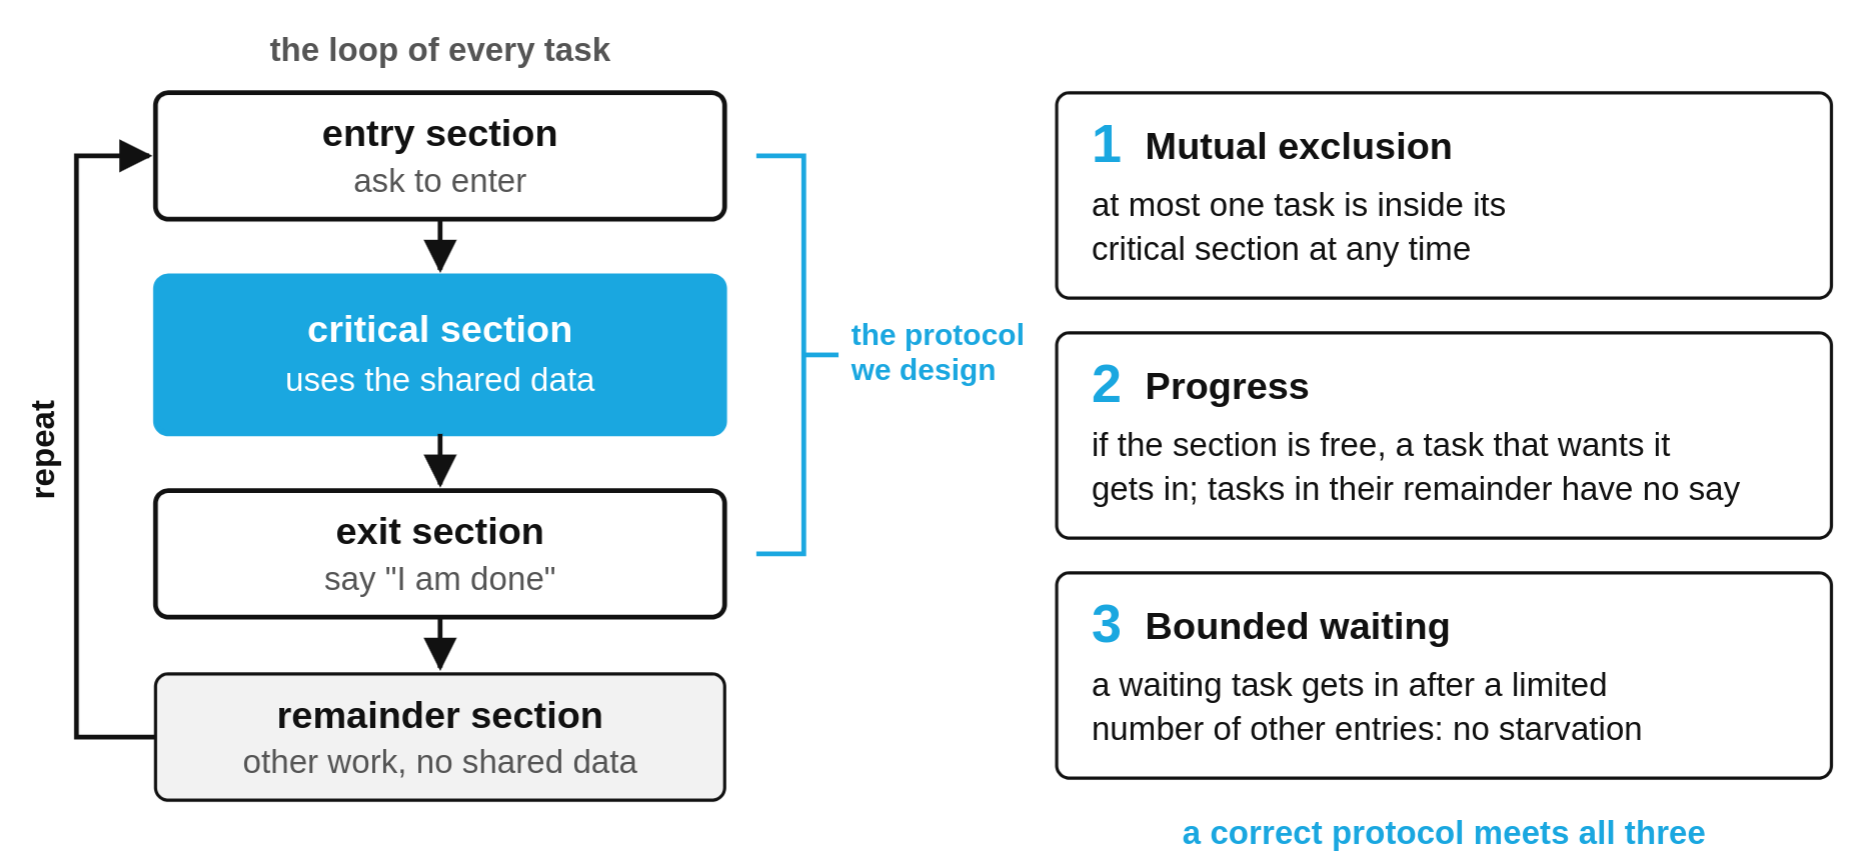
\includegraphics[scale=0.22]{../figures/crit.png}
\end{center}

We see that whatever protocol we define must meet:
\begin{itemize}
	\item \textbf{Mutual exclusion}: at most one task is inside its critical section at any time. This is the whole point of the protocol;
	\item \textbf{Progress}: if nobody is inside and some tasks want to enter, one of them gets in; a task busy in its remainder section cannot stop them. A protocol that keeps the door always closed is safe but useless;
	\item \textbf{Bounded waiting}: once a task asks to enter, the other tasks can enter only a limited number of times before it does. Otherwise it may starve.
\end{itemize}

We assume nothing about speed: the protocol must work for any interleaving, any quantum, any number of interrupts.

Let's see a few possible solutions.

\subsubsection{Mask interrupts}

On one CPU, a task loses the CPU only in two ways: an interrupt (the tick, then PendSV), or its own call (\texttt{yield()}, \texttt{sleep()}, ...). If the critical section masks interrupts and makes no such call, no other task can run inside it.

This, though, is quite limited and applies to small things we basically alerady saw, \textit{inside} the kernel:
\begin{itemize}
	\item 
\textbf{Privileged only}: \texttt{cpsid i} changes PRIMASK only in privileged mode. Our tasks are unprivileged, and in unprivileged mode the instruction is simply ignored: no fault, no effect. That is on purpose: a task that could mask interrupts could stop the tick and keep the CPU for ever, and the whole protection layer would be useless; 
	\item
\textbf{Latency}: while interrupts are masked, every interrupt waits, even an urgent one that has nothing to do with the shared data. The section must be very short;
	\item
\textbf{One CPU} only: on a chip with two cores, masking on core 0 does nothing to core 1, which keeps running and can enter the same section at the same time.
\end{itemize}

So masking is a good tool inside the kernel, for a few instructions. Tasks need something else: we can't give them access to interrupt masking as is.

\subsubsection{Test-and-set flags}

A shared flag in memory is useless as it suffers from the exact problem we're trying to solve.
We can do with some hardware help. 
The fix needs the read and the write of the flag to be one atomic step: an atomic read-modify-write.
The classic one is \textbf{test-and-set}: in one step, read the old value of a word and write 1 into it.

If test-and-set returns 0, the word was free and you set it: you hold the lock. If it returns 1, someone else holds it, and your write of 1 changed nothing.
Two tasks can no longer both see 0: the first one's read and write happen together.
Many CPUs have such an instruction (x86 has \texttt{xchg}, which swaps a register and a word). The Cortex-M3 has none: it does it in another way.

The Cortex-M3 splits the atomic step into two instructions that work together:
\begin{lstlisting}[language=arm, style=codestyle]	
ldrex r1, [r0]     @ r1 = *r0, and start watching: "exclusive access begins"
strex r2, r1, [r0] @ if nothing happened since ldrex: *r0 = r1, r2 = 0
                   @ else: store nothing, r2 = 1 (failed)
\end{lstlisting}

\begin{itemize}
	\item \texttt{ldrex} (\textit{load exclusive}) is a normal load that also says "I want to update this word";
	\item \texttt{strex} (\textit{store exclusive}) stores only if nothing could have touched the word since the ldrex ; its first register tells you if it did (0) or not (1).
\end{itemize}

If \texttt{strex} fails, you simply start again from the \texttt{ldrex}-
Between the two you can compute anything: test the old value, add 1, ... So the pair gives test-and-set, an atomic increment, and more.

The exclusiveness is ensured by a small piece of hardware: the \textbf{exclusive monitor}.

\begin{center}
	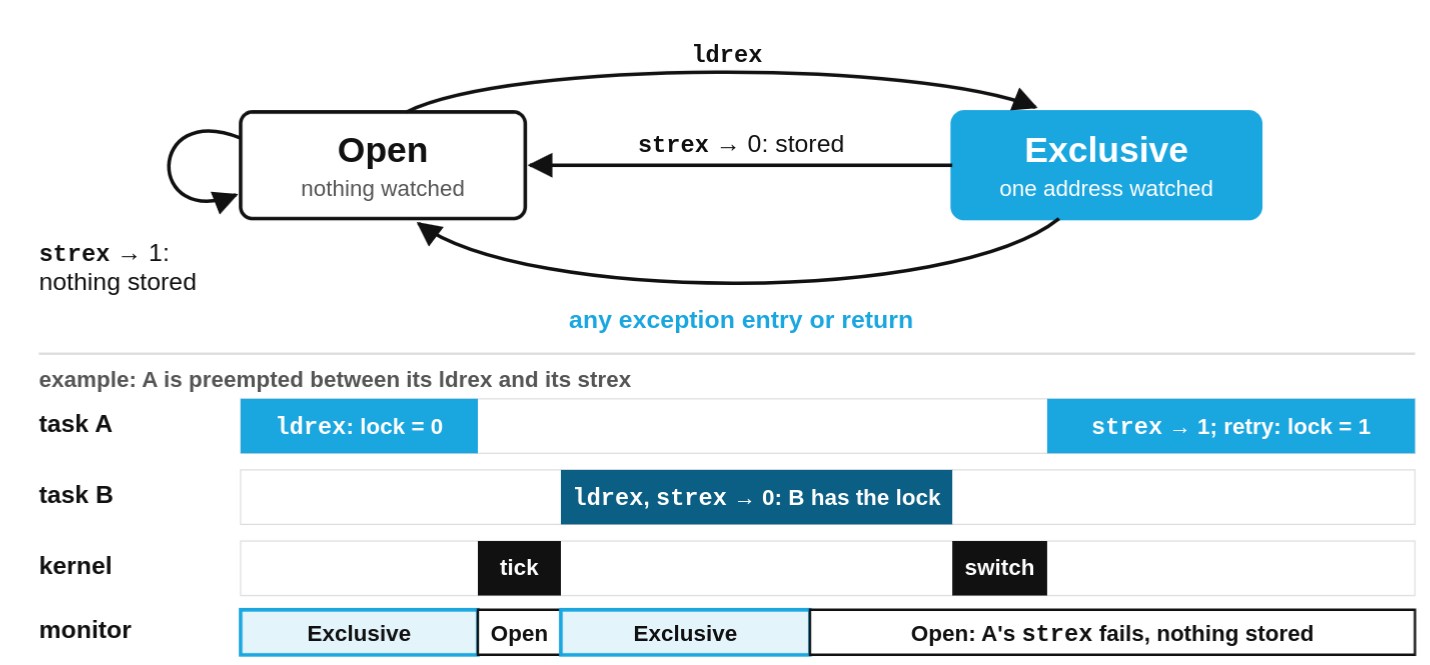
\includegraphics[scale=0.22]{../figures/exc_mon.png}
\end{center}

Two states, \textit{Open} and \textit{Exclusive}: \texttt{ldrex} sets Exclusive; \texttt{strex} stores only in Exclusive, then sets Open.
Any exception entry or return sets it to Open (tick, UART interrupt, PendSV, system call), even without a switch.
On one CPU another task runs only after an exception: a preempted \texttt{strex} fails and A retries.

\par\smallskip

Another thing to note: to be fast, a CPU and its memory system may let memory accesses complete in a different order than in the program (on bigger cores than ours, very often; the compiler may reorder them too).
For a lock that would be fatal: a write of the critical section could become visible after the unlock store, when another task already holds the lock.

\texttt{dmb} (\textit{data memory barrier}) allows use to fence this: every memory access before it completes before any memory access after it.
The rule is to fence on memory after taking the lock (the section's accesses cannot move before it) and before releasing it. (they cannot move after it).
On one Cortex-M3 the barrier costs almost nothing and rarely changes anything, but with it the lock stays correct on every ARM core.

\par\smallskip

What we implemented is basically a \textbf{spinlock}: while the lock is taken, the task stays in its loop and tries again and again.
Waiting by looping on the CPU is busy waiting: it can be done by unprivileged tasks, but it's also really wasteful.

If we have the right primitives available, it's better to do \textbf{spin-then-yield}.
That is, if the lock is taken, yield the task: the holder runs, frees the lock, and you try again at your next turn.

\subsubsection{Semaphores}

A \textbf{semaphore} $S$ is an integer counter, plus a list of tasks blocked on it. It has two operations, both atomic:
\begin{itemize}
	\item \textbf{Wait}: if $S$'s count is above zero, subtract one from it. Otherwise block on the blocked list;
	\item \textbf{Signal}: if the blocked list holds blocked tasks, free the oldest one. Otherwise add one from $S$'s count.
\end{itemize}

\par\smallskip

A \textbf{mutex} (from \textit{mutual exclusion}) is a lock with an owner: the task that locked it is the only one allowed to unlock it.
Two operations:
\begin{itemize}
	\item \textbf{Lock}: if free, the caller becomes the owner; if taken, the caller waits (usually blocked, like a semaphore);
	\item \textbf{Unlock}: allowed only to the owner; the next waiting task becomes the owner. An unlock by another task is an error the kernel can report.
\end{itemize}

If you think about it hard enough, kernel-side a mutex is just a semaphore initialized at one and where only who moves past the wait is allowed to signal.
User-side we need stronger semantics.

\end{document}
